
\documentclass[runningheads]{llncs}

% ==========================================
% PAQUETES
% ==========================================
\usepackage[utf8]{inputenc}
\usepackage[T1]{fontenc}
\usepackage[spanish]{babel}
\usepackage{graphicx}
\usepackage[spanish,es-tabla]{babel}
\usepackage{amsmath,amssymb}
\usepackage{booktabs}
\usepackage{xcolor}
\usepackage{listings}
\usepackage{float}
\usepackage{array}
\usepackage{pgfplots}
\pgfplotsset{compat=1.18}

% p==========================================
% FORMATO DEL CODIGO JAVA
% ==========================================
\lstdefinestyle{javaStyle}{
    language=Java,
    basicstyle=\ttfamily\scriptsize,
    keywordstyle=\color{blue},
    commentstyle=\color{gray},
    stringstyle=\color{red!70!black},
    numbers=left,
    numberstyle=\tiny\color{gray},
    breaklines=true,
    frame=single,
    showstringspaces=false,
    tabsize=4
}

\begin{document}

% ==========================================
% PORTADA
% ==========================================
\begin{titlepage}
    \thispagestyle{empty}
    \centering

    \vspace*{0.3cm}

    % Primera imagen
    \begin{minipage}[c][2.8cm][c]{0.42\textwidth}
        \centering
        \IfFileExists{epn.png}{
            
\includegraphics[
                width=\linewidth,
                height=2.7cm,
                keepaspectratio
            ]{epn.png}
        }{
            \fbox{
                \parbox[c][2.2cm][c]{0.85\linewidth}{
                    \centering Imagen 1
                }
            }
        }
    \end{minipage}
    \hfill
    % Segunda imagen
    \begin{minipage}[c][2.8cm][c]{0.42\textwidth}
        \centering
        \IfFileExists{fis.jpg}{
            
\includegraphics[
                width=\linewidth,
                height=2.7cm,
                keepaspectratio
            ]{fis.jpg}
        }{
            \fbox{
                \parbox[c][2.2cm][c]{0.85\linewidth}{
                    \centering Imagen 2
                }
            }
        }
    \end{minipage}

    \vspace{1.0cm}

    {\LARGE\bfseries
    Escuela Politécnica Nacional\par}

    \vspace{0.5cm}

    {\large
    Ing. en Ciencia de Datos e Inteligencia Artificial\par}

    \vspace{1.0cm}


    {\large\bfseries
    Benchmarking de Rendimiento y Análisis de Complejidad con Spring Boot y JMeter\par}

    \vspace{1.0cm}

    {\Large\bfseries
    Estructura de Datos y Algoritmos II\par}

    \vspace{0.65cm}

    {\large\bfseries Integrantes\par}

    \vspace{0.3cm}

    Aitana Gomez\\[0.2cm]
    Juan Jacome\\[0.2cm]
    Matias Monge\\[0.2cm]
    Alejandro Villacis

    \vspace{0.65cm}

    {\large\bfseries Docente\par}

    \vspace{0.15cm}

    Ing. David Galarza

    \vspace{0.45cm}

    {\large\bfseries Fecha\par}

    \vspace{0.15cm}

    16 de octubre del 2026

    \vfill
\end{titlepage}


% -------------------------------------------------
\section{Introducción}
% -------------------------------------------------

La notación Big O permite describir el crecimiento
asintótico del costo de un algoritmo, considerando
principalmente su comportamiento cuando el tamaño
de la entrada aumenta. Entre las complejidades más
comunes se encuentran la lineal, $O(n)$, y la
cuadrática, $O(n^2)$.

El objetivo de este trabajo es comparar estos dos métodos
desarrollados con Java y Spring Boot, uno basado en
un único bucle y otro basado en dos bucles anidados.
La evaluación se realiza desde dos perspectivas:
el análisis teórico de las operaciones y la medición
empírica del tiempo de respuesta mediante Apache
JMeter.

La pregunta central es cómo se relaciona la
complejidad temporal de ambos métodos con el
rendimiento observado durante las pruebas HTTP.

\begin{itemize}
    \item Objetivo: Evaluar de forma empírica y teórica el impacto de la complejidad algorítmica 
    $O(n)$ y $O(n^2)$ en el rendimiento de una aplicación backend mediante pruebas de carga automatizadas, documentando los hallazgos en un informe científico formal.
\end{itemize}

% -------------------------------------------------
\section{Fundamento teórico}
% -------------------------------------------------

\subsection{Notación Big O}

La notación Big O caracteriza una cota asintótica
superior del crecimiento de una función. Una función
$f(n)$ pertenece a $O(g(n))$ si existen constantes
positivas $c$ y $n_0$ tales que

\begin{equation}
0 \leq f(n) \leq c g(n),
\qquad n \geq n_0.
\end{equation}

En el análisis de algoritmos, se utiliza esta
notación para estudiar cómo aumenta el número de
operaciones relevantes al incrementar el tamaño
de la entrada, omitiendo constantes multiplicativas
y términos de menor orden.

\subsection{Complejidad lineal}

Un algoritmo presenta complejidad temporal lineal
cuando el número de operaciones crece
proporcionalmente al tamaño de entrada $n$.
Un ejemplo es un bucle que recorre una secuencia
de $n$ elementos una sola vez.

Su función de costo puede expresarse como

\begin{equation}
T(n)=an+b,
\end{equation}

donde $a$ representa el costo asociado a cada
iteración y $b$ corresponde a los costos fijos.
Al considerar el término dominante se obtiene

\begin{equation}
T(n) \in O(n).
\end{equation}

\subsection{Complejidad cuadrática}

La complejidad cuadrática aparece, por ejemplo,
cuando un bucle de $n$ iteraciones contiene otro
bucle que también realiza $n$ iteraciones por
cada ejecución del bucle exterior.

El número total de iteraciones es

\begin{equation}
T(n)=n \cdot n=n^2.
\end{equation}

Si se consideran los costos constantes y otras
operaciones, el modelo puede escribirse como

\begin{equation}
T(n)=an^2+bn+c.
\end{equation}

El término dominante es $n^2$, por lo que

\begin{equation}
T(n) \in O(n^2).
\end{equation}

Cuando se duplica el tamaño de entrada, un
algoritmo lineal duplica aproximadamente su
cantidad de iteraciones. En cambio, un algoritmo
cuadrático multiplica por cuatro dicha cantidad.

% -------------------------------------------------
\section{Metodología}
% -------------------------------------------------

\subsection{Diseño experimental}

Utilizamos una aplicación web con Java
y Spring Boot. La aplicación expone dos endpoints
HTTP que permiten ejecutar los métodos bajo prueba.
Posteriormente, se utilizó Apache JMeter para enviar
solicitudes a dichos endpoints y registrar métricas
de rendimiento.

Los dos métodos se evaluaron por separado,
manteniendo como referencia el tamaño de entrada
predeterminado $n=5000$ y un total de 1000 muestras
por prueba, según los reportes obtenidos.

\subsection{Entorno de ejecución}

La Tabla~\ref{tab:entorno} presenta las
características del entorno experimental. Los
campos de hardware deben completarse con las
especificaciones reales del equipo utilizado.

\begin{table}[htbp]
\centering
\caption{Características del entorno experimental.}
\label{tab:entorno}
\begin{tabular}{ll}
\toprule
\textbf{Componente} & \textbf{Configuración} \\
\midrule
Sistema operativo & Windows \\
Lenguaje de programación & Java \\
Framework & Spring Boot \\
Herramienta de pruebas & Apache JMeter 5.6.3 \\
Tamaño de entrada & $n=5000$ \\
Muestras por prueba & 1000 \\
Procesador & AMD Ryzen 9 270 w/ Radeon 780M Graphics (4.00 GHz) \\
Memoria RAM & 32.0 gb \\
Versión de Java & JDK 25 \\
Versión de Spring Boot & Mas actualizada \\
\bottomrule
\end{tabular}
\end{table}

Para asegurar la reproducibilidad, es necesario
registrar también la configuración del grupo de
hilos de JMeter, el periodo de subida, el número
de usuarios concurrentes, la duración de la prueba
y las condiciones de ejecución del servidor.

\subsection{Algoritmo lineal}

El primer endpoint es \texttt{/api/benchmark/optimizado}.
Su implementación contiene un único bucle:

\begin{verbatim}
long sumaTotal = 0;

for (int indice = 0; indice < n; indice++) {
    sumaTotal += indice % 3;
}
\end{verbatim}

El índice toma los valores desde $0$ hasta $n-1$.
Por consiguiente, el cuerpo del bucle se ejecuta
exactamente $n$ veces. Para $n=5000$, se realizan
5000 iteraciones.

Si cada iteración tiene un costo constante,
el número de operaciones se expresa como

\begin{equation}
T_L(n)=an+b.
\end{equation}

Por lo tanto, la complejidad temporal es

\begin{equation}
\boxed{T_L(n)\in O(n)}.
\end{equation}

\subsection{Algoritmo cuadrático}

El segundo endpoint es
\texttt{/api/benchmark/ineficiente}. Su implementación
utiliza dos bucles anidados:

\begin{verbatim}
long sumaTotal = 0;

for (int fila = 0; fila < n; fila++) {
    for (int col = 0; col < n; col++) {
        sumaTotal += (fila + col) % 3;
    }
}
\end{verbatim}

El bucle exterior se ejecuta $n$ veces. Para cada
iteración exterior, el bucle interior también se
ejecuta $n$ veces. En consecuencia, el número total
de ejecuciones del cuerpo interior es

\begin{equation}
T_C(n)=\sum_{i=1}^{n} n=n^2.
\end{equation}

Para el tamaño de entrada utilizado en el
experimento se obtiene

\begin{equation}
T_C(5000)=5000^2=25\,000\,000.
\end{equation}

El modelo de costo se puede expresar como

\begin{equation}
T_C(n)=an^2+bn+c,
\end{equation}

y su complejidad temporal es

\begin{equation}
\boxed{T_C(n)\in O(n^2)}.
\end{equation}

\subsection{Diferencia entre las implementaciones}

Aunque ambos métodos se utilizan para comparar
complejidades, no son implementaciones equivalentes
del mismo cálculo. El método lineal acumula
\texttt{indice \% 3}, mientras que el cuadrático
acumula \texttt{(fila + col) \% 3}.

Por tanto, la comparación permite estudiar el
comportamiento de dos cargas computacionales con
diferente complejidad, pero no demostrar que una
implementación sea una optimización funcionalmente
equivalente de la otra.

% -------------------------------------------------
\section{Resultados experimentales}
% -------------------------------------------------

\subsection{Resultados del algoritmo lineal}

La primera ejecución corresponde al endpoint
\texttt{/api/benchmark/optimizado}. En la
Figura~\ref{fig:optimizado} se reserva el espacio
para incorporar el reporte resumen de Apache JMeter.

\begin{figure}[htbp]
\centering
\IfFileExists{IMG-20261016-WA0002.jpg}{
    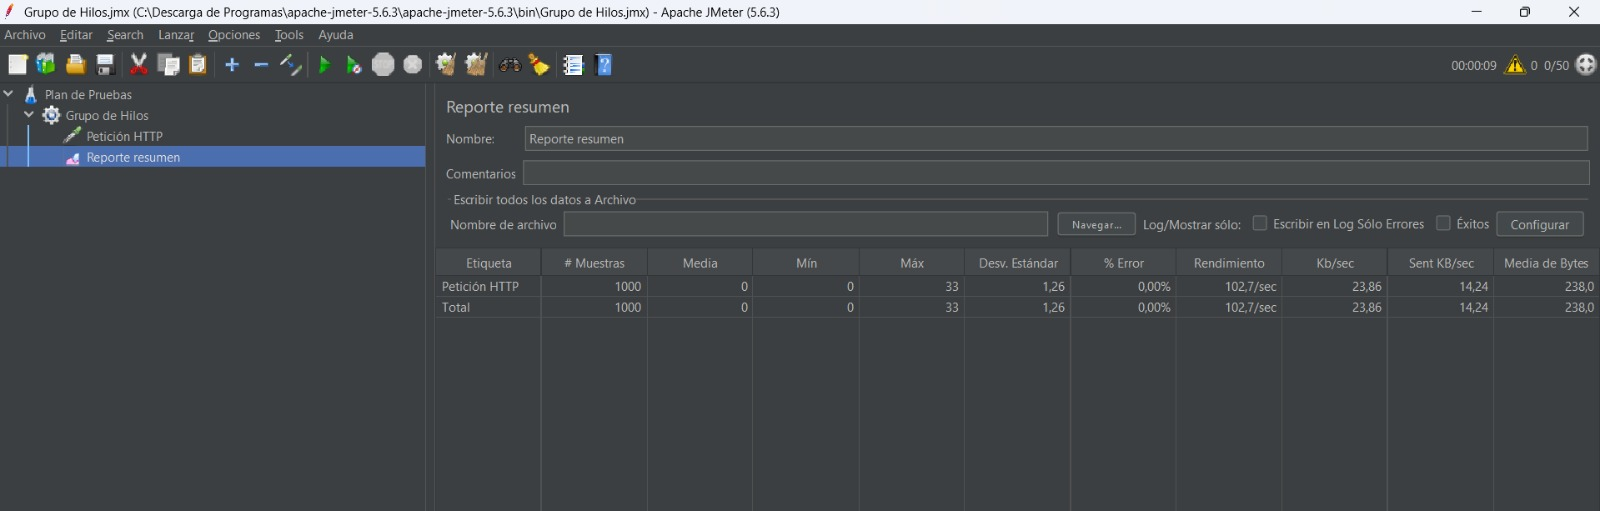
\includegraphics[width=\linewidth]
    {IMG-20261016-WA0002.jpg}
}{
    \fbox{\parbox[c][5cm][c]{0.90\linewidth}{
    \centering
    Espacio reservado para la captura del reporte
    de JMeter del algoritmo optimizado.\\
    Archivo: \texttt{jmeter\_optimizado.png}
    }}
}
\caption{Reporte resumen de Apache JMeter para
el algoritmo lineal $O(n)$.}
\label{fig:optimizado}
\end{figure}

El reporte registra 1000 muestras, una media
mostrada de $0$ ms, un mínimo de $0$ ms, un máximo
de $33$ ms y una desviación estándar de $1{,}26$ ms.
El porcentaje de errores es $0{,}00\%$ y el
rendimiento informado es de $102{,}7$ solicitudes
por segundo.

La media presentada como cero no implica que la
ejecución haya tardado literalmente cero tiempo.
El valor puede estar redondeado por la
representación en milisegundos enteros de JMeter.
Por ello, se requiere una herramienta de medición
de mayor resolución para caracterizar con precisión
tiempos de ejecución tan pequeños.

\subsection{Resultados del algoritmo cuadrático}

La segunda ejecución corresponde al endpoint
\texttt{/api/benchmark/ineficiente}. La
Figura~\ref{fig:ineficiente} permite incorporar
el segundo reporte resumen.

\begin{figure}[htbp]
\centering
\IfFileExists{IMG-20261016-WA0005.jpg}{
    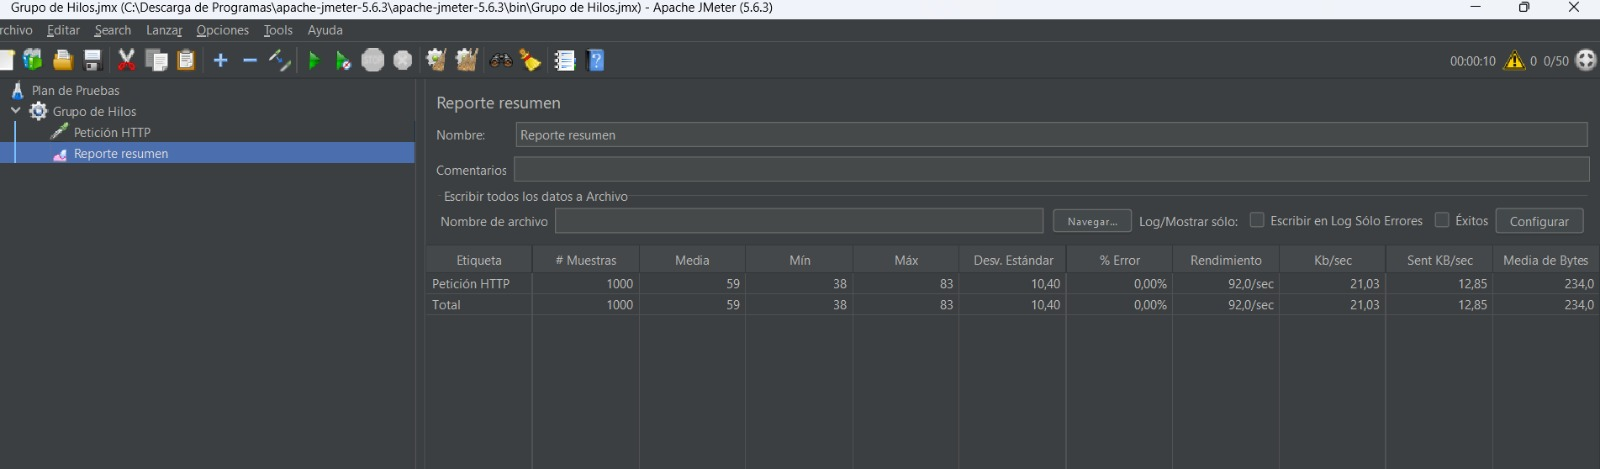
\includegraphics[width=\linewidth]
    {IMG-20261016-WA0005.jpg}
}{
    \fbox{\parbox[c][5cm][c]{0.90\linewidth}{
    \centering
    Espacio reservado para la captura del reporte
    de JMeter del algoritmo ineficiente.\\
    Archivo: \texttt{jmeter\_ineficiente.png}
    }}
}
\caption{Reporte resumen de Apache JMeter para
el algoritmo cuadrático $O(n^2)$.}
\label{fig:ineficiente}
\end{figure}

En esta ejecución se registraron 1000 muestras,
una media de $59$ ms, un mínimo de $38$ ms, un
máximo de $83$ ms y una desviación estándar de
$10{,}40$ ms. El porcentaje de errores también
fue de $0{,}00\%$, mientras que el rendimiento
observado fue de $92{,}0$ solicitudes por segundo.

La media superior es consistente con la mayor
cantidad de operaciones realizadas por el método
cuadrático. Sin embargo, el tiempo medido por
JMeter corresponde a la solicitud HTTP completa,
por lo que también incluye costos de comunicación,
procesamiento del servidor y otros factores del
entorno.

\subsection{Comparación cuantitativa}

La Tabla~\ref{tab:resultados} resume las métricas
observadas en ambas pruebas.

\begin{table}[htbp]
\centering
\caption{Comparación de los resultados registrados
por Apache JMeter.}
\label{tab:resultados}
\begin{tabular}{lrr}
\toprule
\textbf{Métrica} & \textbf{Lineal} &
\textbf{Cuadrático} \\
\midrule
Complejidad temporal & $O(n)$ & $O(n^2)$ \\
Número de muestras & 1000 & 1000 \\
Media (ms) & 0 & 59 \\
Mínimo (ms) & 0 & 38 \\
Máximo (ms) & 33 & 83 \\
Desviación estándar (ms) & 1,26 & 10,40 \\
Errores (\%) & 0,00 & 0,00 \\
Rendimiento (solicitudes/s) & 102,7 & 92,0 \\
Iteraciones para $n=5000$ & 5000 &
25\,000\,000 \\
\bottomrule
\end{tabular}
\end{table}

La diferencia absoluta entre las medias presentadas
es de

\begin{equation}
\Delta \overline{t}=59-0=59\text{ ms}.
\end{equation}

No resulta adecuado calcular una razón entre ambas
medias, debido a que la media del algoritmo lineal
se muestra como cero. El valor presentado puede
ser producto del redondeo y no constituye una
medición exacta del tiempo real.

La diferencia de rendimiento observada es

\begin{equation}
\Delta R=102{,}7-92{,}0
=10{,}7\text{ solicitudes/s}.
\end{equation}


% -------------------------------------------------
\section{Conclusiones}
% -------------------------------------------------

El análisis teórico permitió establecer que el
método basado en un único bucle presenta
complejidad temporal $O(n)$, mientras que el
método con dos bucles anidados presenta
complejidad $O(n^2)$. Para $n=5000$, el primero
realiza 5000 iteraciones y el segundo 25 millones,
lo que evidencia una diferencia sustancial en
la cantidad de operaciones.

Los resultados de Apache JMeter fueron consistentes
con la tendencia esperada: la prueba lineal
registró una media presentada de $0$ ms y un
rendimiento de $102{,}7$ solicitudes por segundo,
mientras que la cuadrática presentó una media de
$59$ ms y un rendimiento de $92{,}0$ solicitudes
por segundo. Ambos ensayos registraron un
porcentaje de errores de $0\%$.

Sin embargo, las mediciones deben interpretarse
con cautela. La media de cero milisegundos no
representa necesariamente un tiempo nulo, y la
latencia HTTP incluye factores adicionales al
tiempo de ejecución del algoritmo. Asimismo,
los dos métodos implementados realizan cálculos
diferentes, por lo que no constituyen versiones
funcionalmente equivalentes.


ENLACE GIT HUB: https://github.com/Slinkypal/EDA-2-Grupo-8


\end{document}